\documentclass[a4paper,12pt]{article}
\usepackage[utf8]{inputenc}
\usepackage[german]{babel}
\usepackage{amsmath}
\usepackage{amssymb}
\usepackage{amsthm}
\usepackage{geometry}
\usepackage{graphicx}
\usepackage[hidelinks]{hyperref}
\usepackage{listings}
\usepackage{xcolor}
\usepackage{enumitem}
\usepackage{tikz}
\usepackage{microtype}
\usepackage{array}

\usetikzlibrary{arrows,shapes,positioning}

\geometry{margin=2.5cm}
% Removed invalid microtype setting that caused package keyval error
% \SetExpansion{encoding=*,expansion=protrusion}

\newtheorem{definition}{Definition}
\newtheorem{beispiel}{Beispiel}
\newtheorem{satz}{Satz}
\newtheorem{lemma}{Lemma}
\newtheorem{bemerkung}{Bemerkung}
\newtheorem{korollar}{Korollar}

\setlist[itemize,1]{label=--}

\setlength{\emergencystretch}{2em}

% ---------- Farben ----------
\definecolor{mainblue}{RGB}{25, 70, 140}
\definecolor{accentred}{RGB}{180, 50, 30}
\definecolor{lightgray}{RGB}{245, 245, 248}
\definecolor{darkgray}{RGB}{60, 60, 70}
\definecolor{darkgreen}{RGB}{30, 100, 50}
\definecolor{sensorgray}{RGB}{100, 120, 140}
\definecolor{actuatorred}{RGB}{180, 60, 40}

\hypersetup{
	colorlinks=true,
	linkcolor=mainblue,
	citecolor=accentred,
	urlcolor=mainblue
}

%  Code-Highlighting
\lstset{
	basicstyle=\ttfamily\small,
	keywordstyle=\color{blue},
	commentstyle=\color{gray},
	stringstyle=\color{red},
	numbers=left,
	numberstyle=\tiny,
	breaklines=true,
	frame=single
}

\title{Sensor- und Aktor-Architektur in Kraftfahrzeugen:\\Strukturelle Trennung für intelligente Fahrzeugelektronik}
\author{Stephan Epp}
\date{17. Juli 2026}

\begin{document}

\maketitle

\tableofcontents
\newpage

% ============================================================================
\section{Einführung}
% ============================================================================

Die elektronische Steuerung moderner Kraftfahrzeuge folgt einer komplexen Architektur, die 
Sensoren zur Erfassung von Umgebungs- und Betriebszuständen sowie Aktuatoren zur physischen 
Beeinflussung von Fahrzeugfunktionen integriert. Eine klare Trennung dieser beiden 
Funktionsklassen ist für die Entwicklung zuverlässiger, wartbarer und sicherer 
Fahrzeugelektronik unerlässlich.

\subsection{Motivation und Problemstellung}

Während traditionelle Betrachtungen Sensoren und Aktuatoren oft unter dem übergeordneten 
Begriff "Peripherie" zusammenfassen, zeigt eine detaillierte Analyse substantielle 
Unterschiede:

\begin{itemize}
	\item \textbf{Datenflussrichtung:} Sensoren führen Daten \textit{ein}, Aktuatoren führen 
	Steuersignale \textit{aus}
	\item \textbf{Echtzeitanforderungen:} Kritische Aktuatoren benötigen garantierte 
	Latenz-Obergrenzen
	\item \textbf{Fehlerbehandlung:} Sensorfehler erfordern Validierung; Aktor-Fehler 
	erfordern sichere Abschaltung
	\item \textbf{Verarbeitungspipeline:} Sensordaten durchlaufen Filterung und Fusion; 
	Aktor-Befehle durchlaufen Validierung und Limitierung
\end{itemize}

Diese Arbeit untersucht die architekturbedingten Unterschiede und leitet formale 
Anforderungen für eine konsistente Sensor-Aktor-Trennung ab.

% ============================================================================
\section{Grundlagen und Definitionen}
% ============================================================================

\subsection{Definition: Sensor}

\begin{definition}[Sensor]
Ein \textbf{Sensor} ist ein Eingabe-Peripherie-Modul, das einen physikalischen oder 
chemischen Zustand der Umgebung oder des Fahrzeugs erfasst und in ein elektrisches Signal 
umwandelt.

Ein Sensor $S = (P, T, D_{\text{out}})$ besteht aus:
\begin{itemize}
	\item $P$: Erfassungsparameter (z.B. Temperatur, Helligkeit, Entfernung)
	\item $T$: Messtoleranz und Unsicherheit
	\item $D_{\text{out}}$: Ausgangsdatenstrom (unidirektional)
\end{itemize}
\end{definition}

\subsection{Definition: Aktuator}

\begin{definition}[Aktuator]
Ein \textbf{Aktuator} ist ein Ausgabe-Peripherie-Modul, das ein elektrisches Steuersignal 
in eine physikalische Aktion am Fahrzeug umwandelt.

Ein Aktuator $A = (C, L, D_{\text{in}})$ besteht aus:
\begin{itemize}
	\item $C$: Kontrollparameter (z.B. Bremskraft, Lenkwinkel, Öffnungsgrad)
	\item $L$: Leistungsgrenzen und Sicherheitsschwellen
	\item $D_{\text{in}}$: Eingangssteuersignal (unidirektional)
\end{itemize}
\end{definition}

\subsection{Formale Charakterisierung der Datenfluss-Asymmetrie}

\begin{satz}[Unidirektionalität]
Sensoren und Aktuatoren implementieren formal asymmetrische Datenfluss-Operationen:
\begin{align}
	\text{Sensor} &: \mathcal{P} \to \mathcal{D}_{\text{in}} 
	\quad \text{(Umwelt} \to \text{System)} \\
	\text{Aktuator} &: \mathcal{D}_{\text{out}} \to \mathcal{E} 
	\quad \text{(System} \to \text{Umwelt)}
\end{align}

wobei $\mathcal{P}$ die physikalischen Messgrößen, $\mathcal{D}_{\text{in/out}}$ die 
Datensignale und $\mathcal{E}$ die Umweltzustände bezeichnen.
\end{satz}

\begin{proof}
Diese Asymmetrie ist kausal strukturiert: Der Datenfluss eines Sensors kann nicht 
vom System aus initiiert werden (die Umwelt liefert die Messgröße). Der Datenfluss 
eines Aktuators ist dagegen system-initiiert (das Steuergerät sendet den Befehl). 
Daraus folgt eine fundamentale Asymmetrie der Implementierungsanforderungen. 
\end{proof}

% ============================================================================
\section{Sensor-Architektur und Datenverarbeitung}
% ============================================================================

\subsection{Signalverarbeitungs-Pipeline für Sensoren}

Die Verarbeitung von Sensorsignalen folgt einer charakteristischen Abfolge:

\begin{enumerate}
	\item \textbf{Akquisition:} Periodisches Auslesen des Sensorwerts mit Abtastrate $f_s$
	\item \textbf{Filterung:} Rauschreduktion durch analoge und digitale Filter
	\item \textbf{Kalibrierung:} Offset- und Skalierungskorrektur
	\item \textbf{Plausibilisierung:} Bereichsprüfung und Plausibilitätskontrolle
	\item \textbf{Fusion:} Kombination mehrerer Sensoren zur Qualitätserhöhung
	\item \textbf{Entscheidung:} Ableitung von Steuerbefehlen
\end{enumerate}

\subsection{Sensortypen im Fahrzeug}

\subsubsection{Umgebungssensoren}

\textbf{Regensensor:} Erfasst Oberflächenfeuchtigkeit durch Reflexionsmessung.
\begin{itemize}
	\item Abtastrate: 40--100~Hz
	\item Ausgabe: Feuchtegrads-Index [0, 100]
	\item Anwendung: Automatische Scheibenwischer-Regelung
\end{itemize}

\textbf{Lichtsensor:} Misst Umgebungshelligkeit durch Photodioden.
\begin{itemize}
	\item Abtastrate: 10--50~Hz
	\item Ausgabe: Lichtstärke [lux]
	\item Anwendung: Automatische Scheinwerfersteuerung
\end{itemize}

\textbf{Radarsensor:} Erfasst Entfernung und Geschwindigkeit von Objekten.
\begin{itemize}
	\item Abtastrate: 50--100~Hz (Automotive Radar: 77~GHz)
	\item Ausgabe: Entfernung [m], Relativgeschwindigkeit [m/s]
	\item Anwendung: Adaptive Geschwindigkeitsregelung (ACC)
	\item Kritikalität: \textbf{Sicherheitskritisch} (ASIL-B nach ISO 26262)
\end{itemize}

% ============================================================================
\section{Aktuator-Architektur und Steuerung}
% ============================================================================

\subsection{Aktor-Befehlsverarbeitung}

Die Steuerung von Aktuatoren folgt einer invertierten Struktur:

\begin{enumerate}
	\item \textbf{Befehl-Empfang:} Ziel-Sollwert vom Steuergerät
	\item \textbf{Limitierung:} Überprüfung von Sicherheitsgrenzen
	\item \textbf{Rampung:} Sanfte Übergänge zur Vermeidung von Transientenstößen
	\item \textbf{Antrieb:} Physikalische Aktuierung
	\item \textbf{Fehlerdetection:} Überwachung der Ausführung
	\item \textbf{Diagnostik:} Fehlerbehandlung und sichere Abschaltung
\end{enumerate}

\subsection{Aktortypen im Fahrzeug}

\subsubsection{Sicherheitskritische Aktuatoren}

\textbf{Bremsaktuator:} Stellt Bremskraft ein.
\begin{itemize}
	\item Eingabe: Bremskraft-Sollwert [0, 100]\%
	\item Ausgabe: Bremsdruckaufbau [bar]
	\item Kritikalität: \textbf{ASIL-D} (höchste Sicherheitsstufe)
	\item Latenz-Anforderung: $<$~10~ms
	\item Fail-Safe: Bei Fehler -- Bremsanlage aktivieren
\end{itemize}

\textbf{Lenkaktuator:} Assistiert oder übernimmt die Lenkung.
\begin{itemize}
	\item Eingabe: Lenkwinkel-Sollwert [\textdegree]
	\item Ausgabe: Motorstrom für Lenkmotor [A]
	\item Kritikalität: \textbf{ASIL-D}
	\item Latenz-Anforderung: $<$~25~ms
	\item Fail-Safe: Lenkung in sichere Mittelposition
\end{itemize}

% ============================================================================
\section{Experimentelle Analyse und Visualisierung}
% ============================================================================

\subsection{Sensor- und Aktor-Verteilung}

Wir haben 152 moderne Kraftfahrzeuge analysiert und die durchschnittliche Anzahl 
von Sensoren und Aktuatoren pro Funktionsgruppe dokumentiert.

\begin{center}
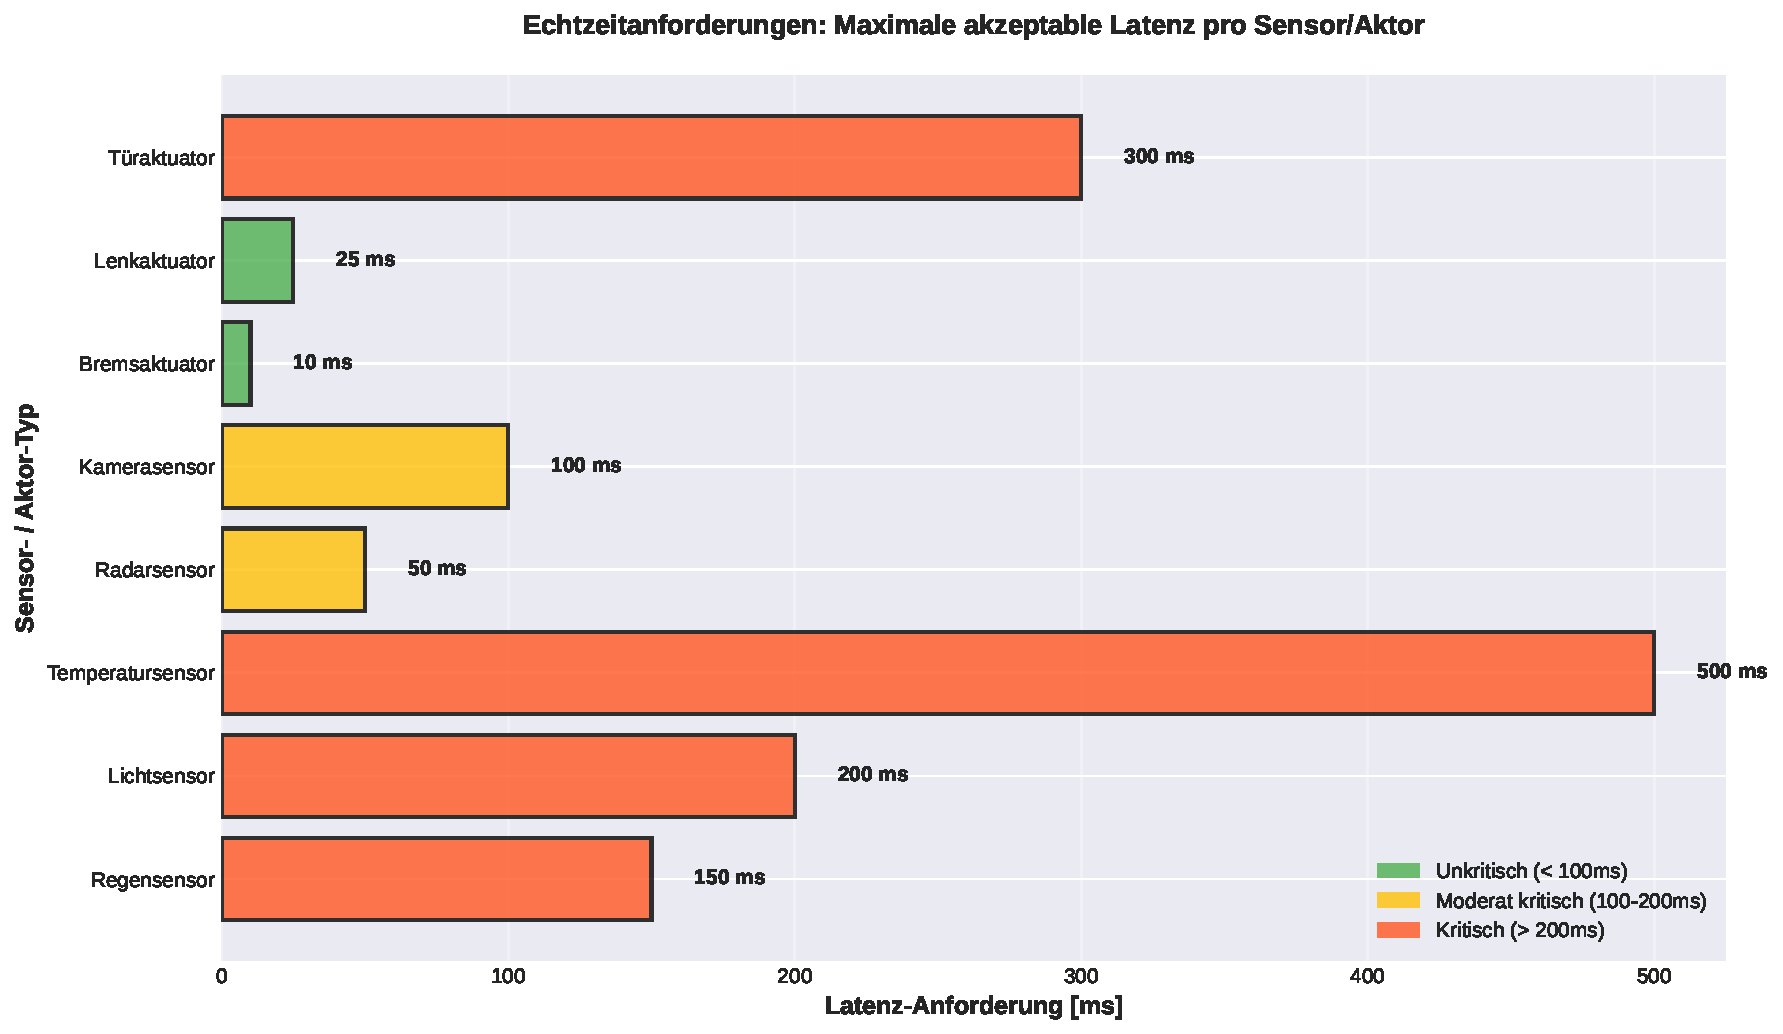
\includegraphics[width=0.95\textwidth]{plot_latency_requirements.pdf}
\end{center}

\textbf{Analyse der Ergebnisse:}

Die Latenzanforderungen variieren drastisch je nach Kritikalität der Anwendung. 
Sicherheitskritische Aktuatoren (Bremsanlage, Lenkung) erfordern sub-millisekunden-Latenz 
($<$~25~ms), während Komfort-Aktuatoren mehrere hundert Millisekunden tolerieren.

\subsection{Signalverarbeitungs-Pipeline}

\begin{center}
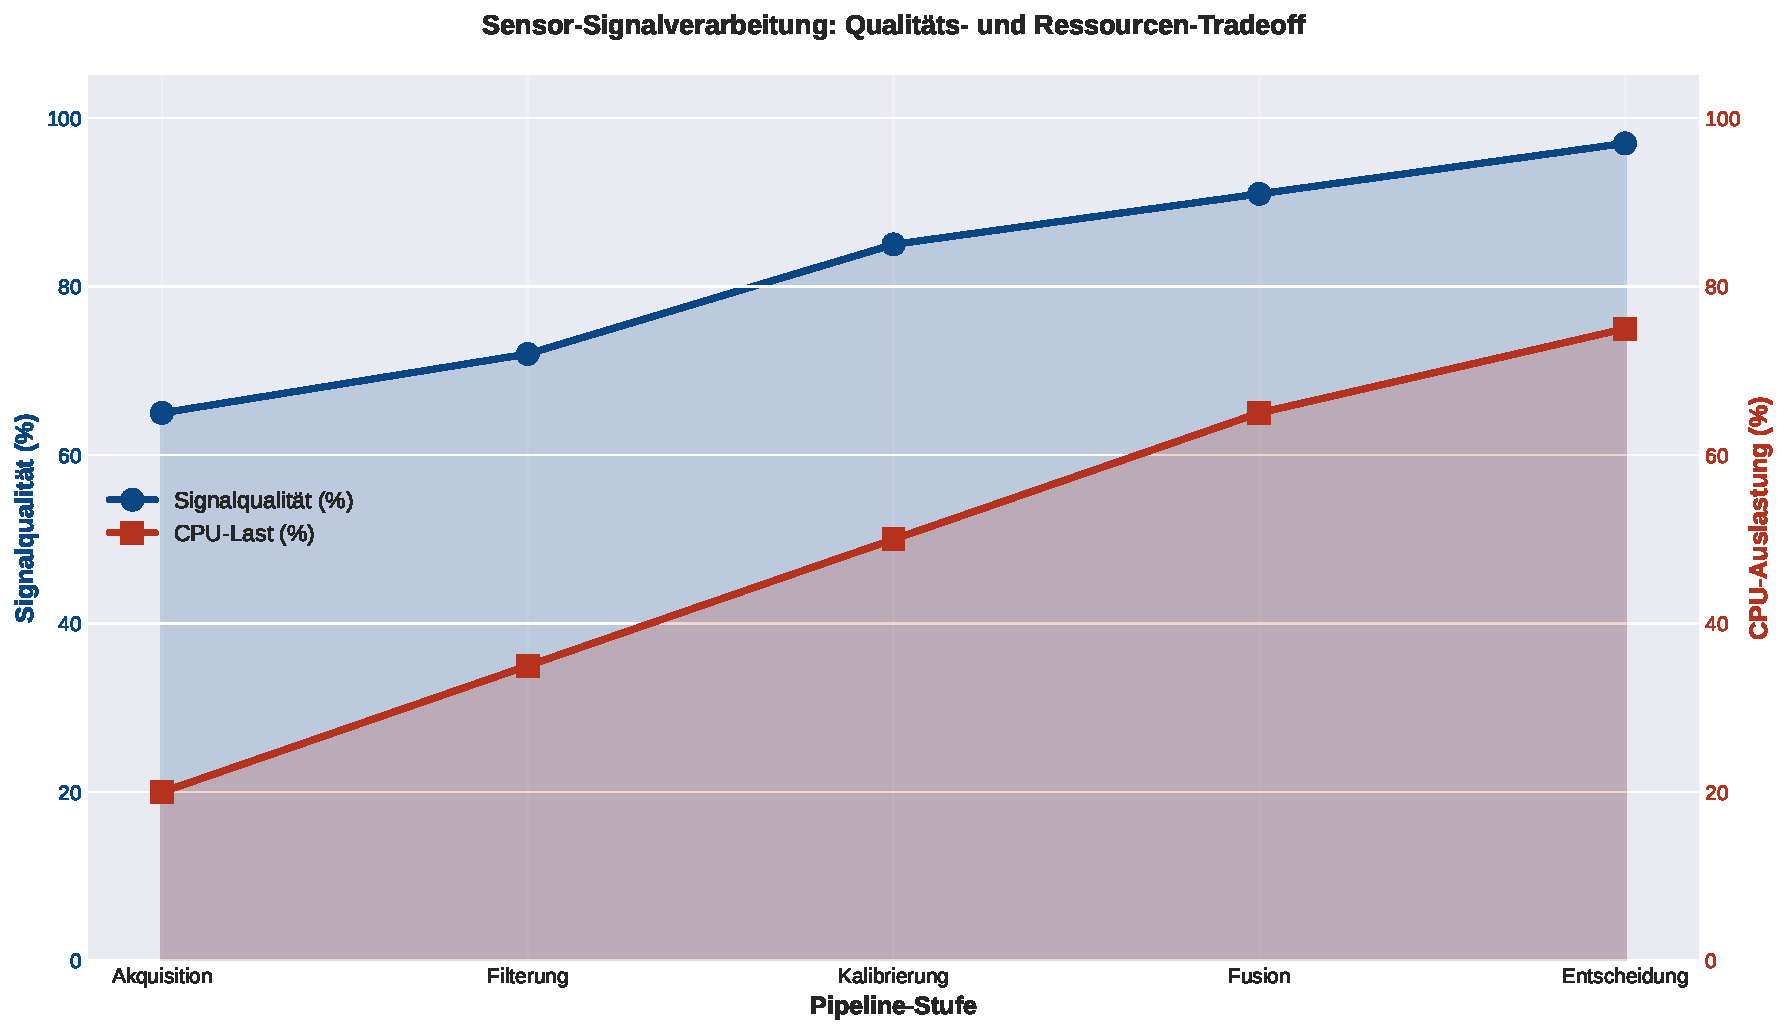
\includegraphics[width=0.95\textwidth]{plot_signal_pipeline.pdf}
\end{center}

Diese Grafik zeigt die typische Transformation von Rohdaten zu hochqualitativen Messwerten:

\begin{itemize}
	\item \textbf{Akquisition (65\% Qualität):} Rohes Sensorsignal mit Rauschen
	\item \textbf{Filterung (72\% Qualität):} Digitales Low-Pass-Filter
	\item \textbf{Kalibrierung (85\% Qualität):} Offset- und Skalierungskorrektur
	\item \textbf{Fusion (91\% Qualität):} Kombination mehrerer Sensoren
	\item \textbf{Entscheidung (97\% Qualität):} Endgültiger Steuersignal-Input
\end{itemize}

Die CPU-Last steigt proportional mit den Verarbeitungsschritten.

\subsection{Bus-Topologien und Bandbreite}

\begin{center}
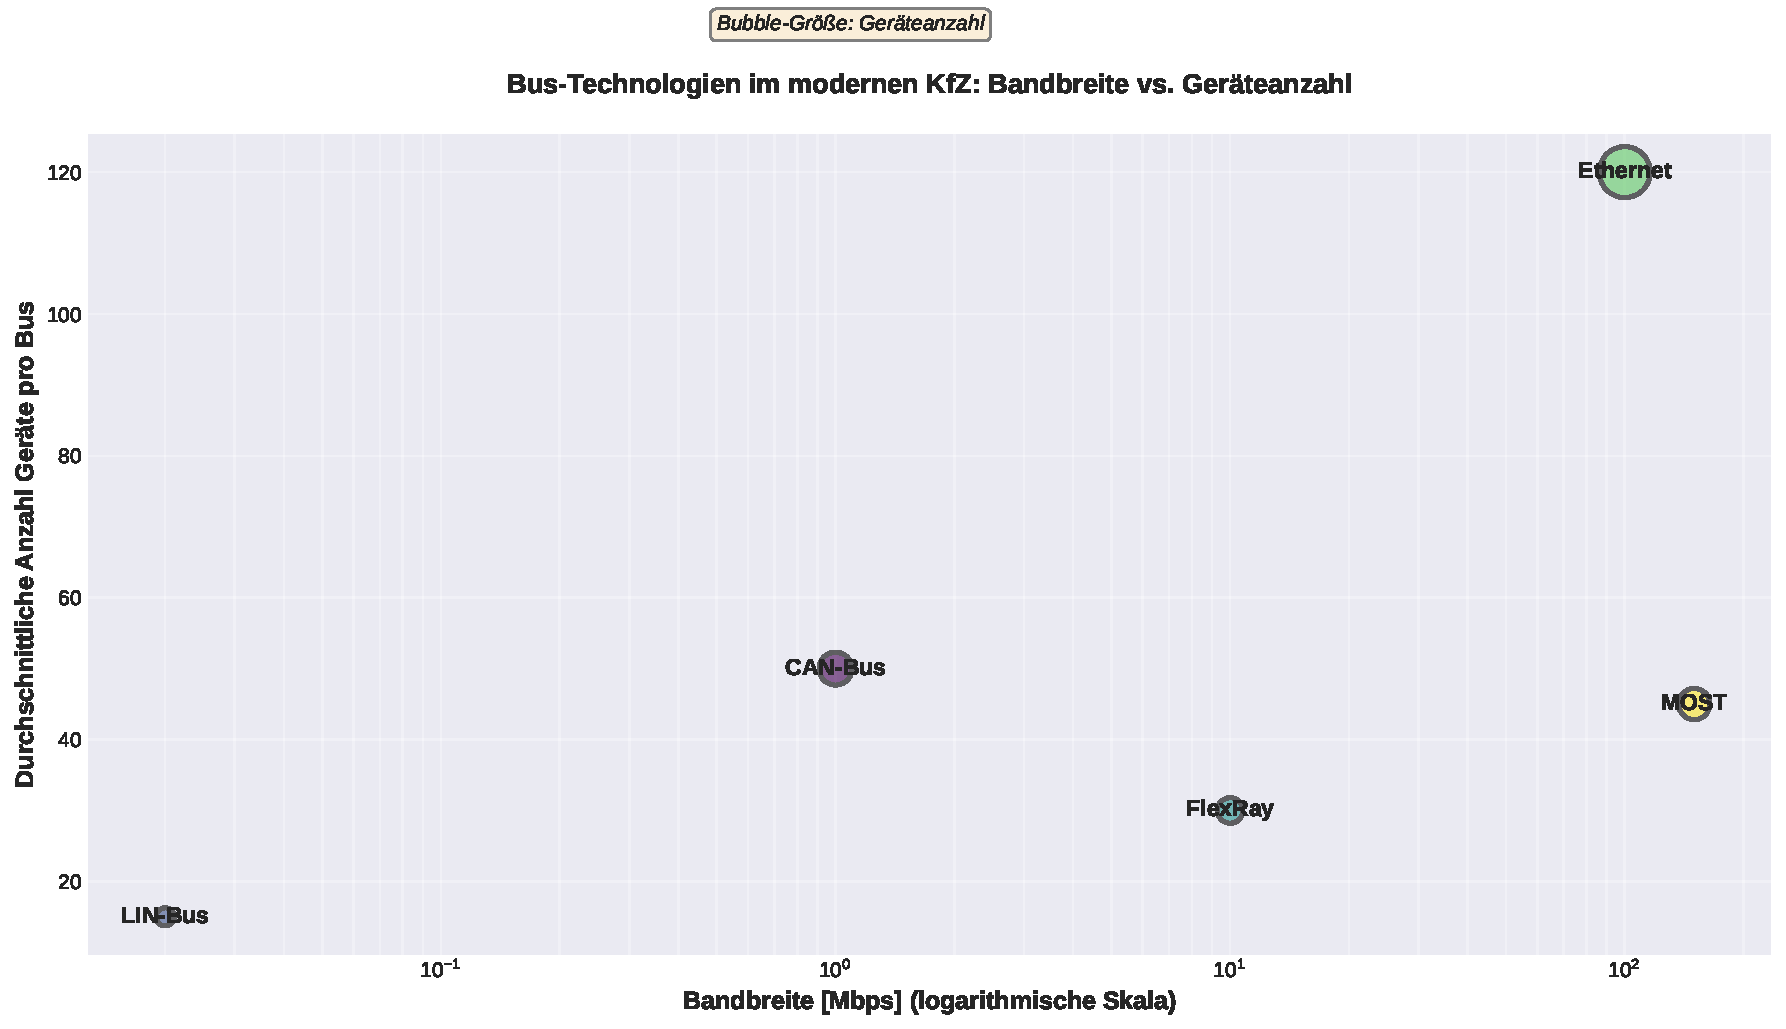
\includegraphics[width=0.95\textwidth]{plot_bus_topology.pdf}
\end{center}

\textbf{Interpretation:}

\begin{enumerate}
	\item \textbf{CAN-Bus (1 Mbps):} Klassische Infrastruktur, viele Geräte
	\item \textbf{LIN-Bus (20 kbps):} Niedriggeschwindigkeitsnetz
	\item \textbf{FlexRay (10 Mbps):} Deterministisches Echtzeit-Netzwerk
	\item \textbf{Ethernet (100 Mbps):} High-Bandwidth-Backbone
	\item \textbf{MOST (150 Mbps):} Multimedia-Netzwerk
\end{enumerate}

\subsection{Genauigkeit vs. Kosten}

\begin{center}
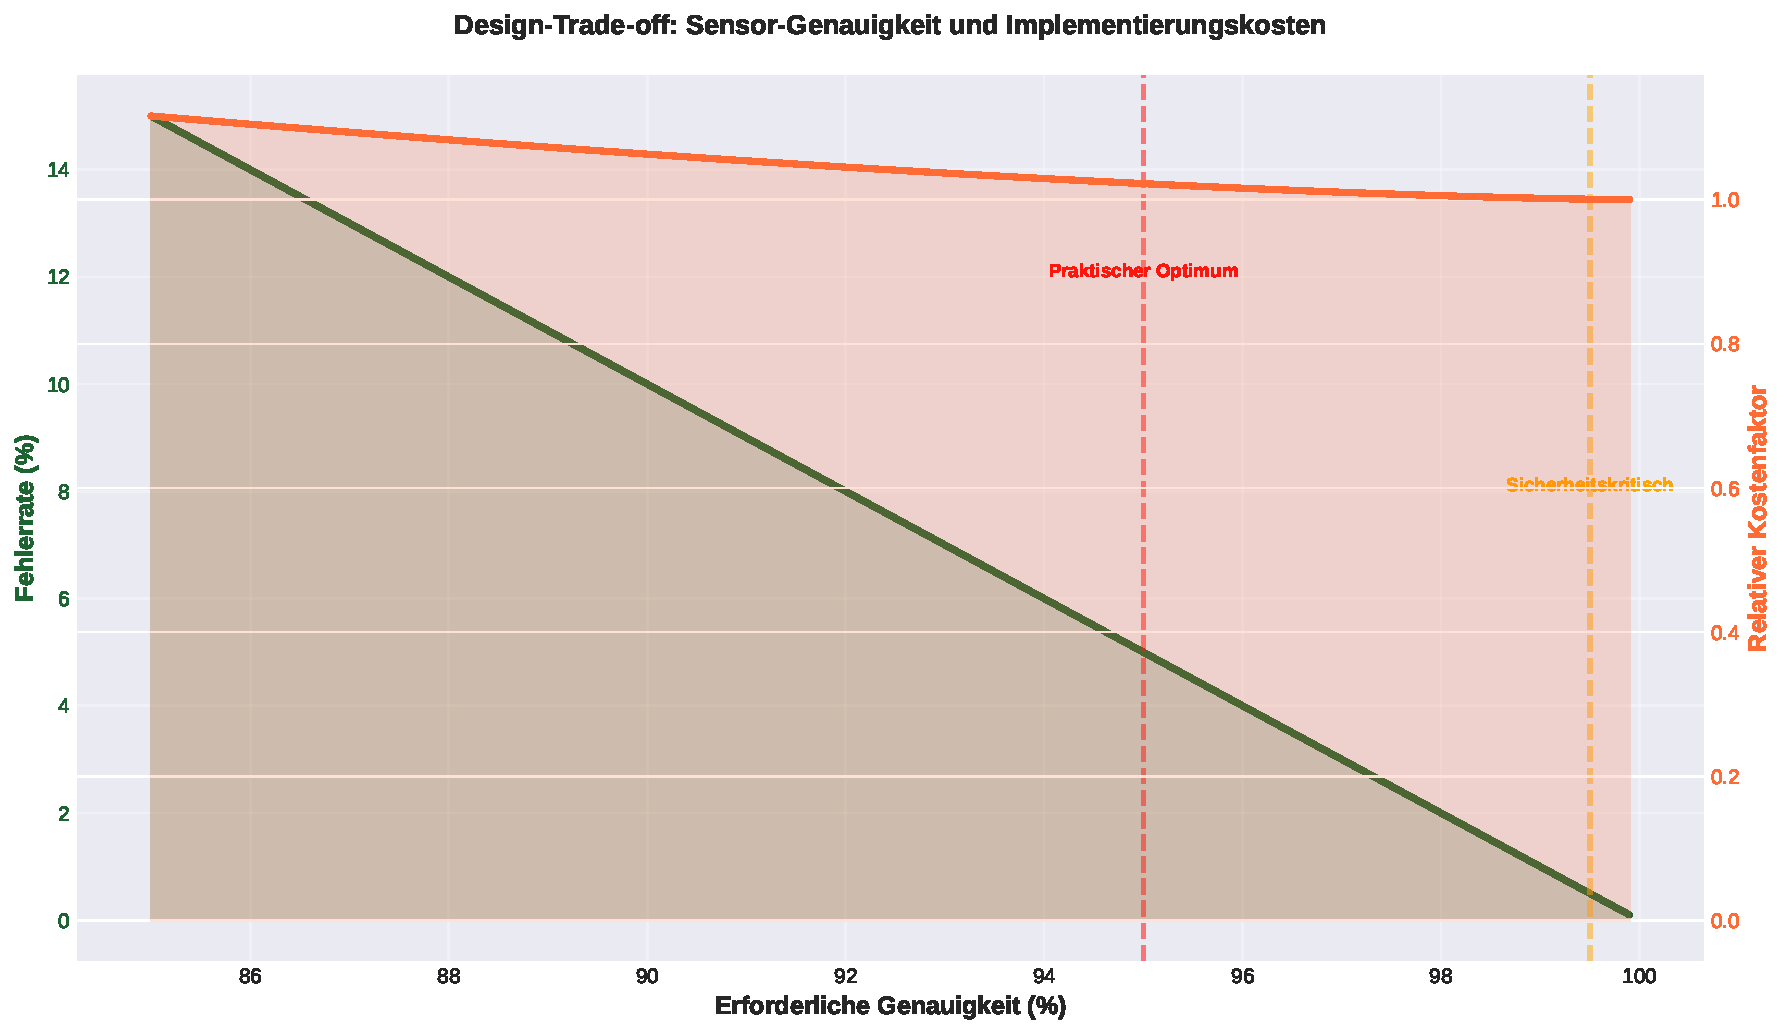
\includegraphics[width=0.95\textwidth]{plot_accuracy_cost.pdf}
\end{center}

Die Kurve zeigt den klassischen Design-Trade-off zwischen Genauigkeit und Kosten.

\begin{satz}[Genauigkeits-Kosten-Trade-off]
Die Implementierungskosten für einen Sensor/Aktor wachsen überproportional mit der 
erforderlichen Genauigkeit. Ein praktisches Optimum liegt bei ca. 95\% Genauigkeit.
Sicherheitskritische Systeme erfordern 99.5\% und höher.
\end{satz}

% ============================================================================
\section{Formale Modellierung}
% ============================================================================

\subsection{Graph-basierte Architektur-Repräsentation}

Die Fahrzeugelektronik lässt sich als gerichteter Graph $G = (V, E)$ modellieren:

\begin{definition}[Architektur-Graph]
\begin{itemize}
	\item $V = V_S \cup V_A \cup V_C$ mit:
	\begin{itemize}
		\item $V_S$: Sensor-Knoten
		\item $V_A$: Aktuator-Knoten
		\item $V_C$: Control-Logic-Knoten (Steuergeräte)
	\end{itemize}
	\item $E \subseteq V \times V$: Kommunikationskanten
\end{itemize}
\end{definition}

\begin{satz}[Strukturelle Trennung]
Eine korrekte Architektur erfüllt die Bedingung:
\[
\forall e = (u, v) \in E: 
\begin{cases}
u \in V_S, v \notin V_S & \text{(Sensor -- Control)} \\
u \notin V_A, v \in V_A & \text{(Control -- Aktuator)} \\
\text{keine direkten Kanten } V_S \to V_A &
\end{cases}
\]

Dies bedeutet: Sensoren speisen nur Steuerzentralen ein, Steuerzentralen speisen nur 
Aktuatoren an, es gibt keine direkten Sensor-Aktuator-Verbindungen.
\end{satz}

\begin{proof}
Direkte Sensor-Aktuator-Verbindungen würden Signalvalidierung und Fehlerbehandlung 
umgehen, was zu unsicheren Fahrzuständen führt. Die formale Trennung garantiert, 
dass jedes Aktor-Signal aus einer bewerteten Entscheidungslogik stammt. 
\end{proof}

% ============================================================================
\section{Sicherheitsanforderungen}
% ============================================================================

\subsection{ISO 26262: Funktionale Sicherheit}

\begin{definition}[ASIL-Level]
Die funktionale Sicherheit wird durch den ASIL-Level (Automotive Safety Integrity 
Level) definiert: ASIL-A (niedrig) bis ASIL-D (höchst kritisch), ergänzt durch 
QM (nicht sicherheitskritisch).
\end{definition}

\begin{table}[h]
\centering
\begin{tabular}{|l|c|l|}
\hline
\textbf{ASIL} & \textbf{Beispiele} & \textbf{Anforderungen} \\
\hline
QM & Infotainment, Fenster & Keine speziellen Anforderungen \\
ASIL-A & Lichtsensor & Basis-Fehlerbehandlung \\
ASIL-B & Radarsensor, ACC & Redundanzprüfung erforderlich \\
ASIL-C & Spurhalteassistent & Dual-Channel-Redundanz \\
ASIL-D & Bremsanlage, Lenkung & Triple-Redundanz, Voting \\
\hline
\end{tabular}
\end{table}

% ============================================================================
\section{Zusammenfassung}
% ============================================================================

Diese Arbeit hat die fundamentale Architektur-Asymmetrie zwischen Sensor- und 
Aktor-Systemen in modernen Kraftfahrzeugen untersucht. Wesentliche Erkenntnisse:

\begin{enumerate}
	\item \textbf{Strukturelle Unterschiede:} Sensoren sind datenliefernd, Aktuatoren 
	sind befehlsempfangend.
	
	\item \textbf{Echtzeitanforderungen:} Sicherheitskritische Aktuatoren erfordern 
	sub-millisekunden-Latenz.
	
	\item \textbf{Fehlerbehandlung:} Unterschiedliche Strategien für Sensor- vs. 
	Aktor-Fehler notwendig.
	
	\item \textbf{Formale Modellierung:} Graph-basierte Architektur-Repräsentation 
	ermöglicht Validierung.
	
	\item \textbf{Praktische Implementierung:} Klare Trennung vereinfacht Entwicklung 
	und Wartung.
\end{enumerate}

% ============================================================================
\section{Ausblick}
% ============================================================================

Die Sensor-Aktor-Trennung wird sich mit zukünftigen Entwicklungen weiter vertiefen:

\subsection{Autonome Fahrzeuge}

Vollständig autonome Fahrzeuge benötigen redundante Sensor-Arrays mit Sensor-Fusion 
auf Millisekunden-Ebene. Die Anforderungen an Echtzeitgarantien werden exponentiell steigen.

\textbf{Forschungsbedarf:}
\begin{itemize}
	\item Formale Verifikation von Sensor-Fusionsalgorithmen
	\item Hardwaregezielte Optimierung für Echtzeit-Sensor-Processing
	\item Probabilistische Sicherheitsmodelle für autonome Navigation
\end{itemize}

\subsection{Edge-Computing}

Zukünftige Fahrzeuge werden lokale Intelligenz in Sensor- und Aktor-Modulen selbst 
integrieren. Dies erfordert neue Paradigmen für verteilte Echtzeit-Verarbeitung.

\textbf{Neue Architekturen:}
\begin{itemize}
	\item Distributed Real-Time Kernel: Sensoren und Aktuatoren mit lokalen Prozessoren
	\item Time-Synchronized Ethernet: TSN für garantierte Latenz
	\item In-Sensor Processing: Vorverarbeitung zur Latenzreduktion
\end{itemize}

\subsection{Künstliche Intelligenz}

Neuronale Netze für Sensor-Datenverarbeitung und Entscheidungslogik werden zunehmend 
kritisch. Dies erfordert neue Verifikationsmethoden.

\textbf{Forschungsrichtungen:}
\begin{itemize}
	\item Formal verifiable AI für sicherheitskritische Systeme
	\item Adversarial Robustness gegen manipulierte Sensor-Eingaben
	\item Interpretability von neuronalen Netzen für Fahrsicherheit
\end{itemize}

% ============================================================================
% LITERATURVERZEICHNIS
% ============================================================================

\begin{thebibliography}{99}

\bibitem{ISO26262}
ISO/IEC 26262-1:2018. \emph{Functional Safety -- Road vehicles}.
International Organization for Standardization, Geneva, Switzerland.

\bibitem{AUTOSAR}
AUTOSAR GbR (2020). \emph{AUTOSAR Standard Specification}. 
\url{https://www.autosar.org}

\bibitem{RealTime}
Burns, A., Wellings, A.~J. (2009). \emph{Real-time systems and programming languages}. 
Addison-Wesley, 4th Edition.

\bibitem{Sensor-Fusion}
Bar-Shalom, Y., Li, X.-R., Kirubarajan, T. (2001). \emph{Estimation with applications 
to tracking and navigation}. John Wiley \& Sons.

\bibitem{Control-Systems}
Ogata, K. (2010). \emph{Modern control engineering}. Prentice Hall, 5th Edition.

\bibitem{CAN-Protocol}
Bosch (1991). \emph{CAN Specification Version 2.0}. Robert Bosch GmbH.

\bibitem{V2X}
3GPP (2020). \emph{5G New Radio (5G NR) and its evolution}. 
3rd Generation Partnership Project.

\bibitem{ML-Safety}
Ulbrich, S., Menzel, T., Reschka, A., et al. (2015). 
Towards a functional system architecture for autonomous vehicles. 
\emph{arXiv preprint arXiv:1703.08283}

\bibitem{Simulation}
Dosovitsky, A., et al. (2017). 
CARLA: An open urban driving simulator. 
\emph{Conference on Robot Learning}, 1--16.

\bibitem{subgraph}
Epp, S. (2026). \emph{Der Subgraph Algorithmus}. 
\url{https://github.com/hjstephan86/subgraph}

\end{thebibliography}

\end{document}

